\documentclass{article}
\usepackage[T1]{fontenc}
\usepackage{tgpagella}
\usepackage{graphicx} % Required for inserting images
\usepackage[dvipsnames]{xcolor}
\usepackage{multirow,array}
\usepackage{float}
\usepackage[spanish,es-nolists]{babel}
\usepackage{amsmath}
\usepackage{hyperref}

% https://ctan.org/pkg/tcolorbox
\usepackage[most]{tcolorbox}

\usepackage{parskip}    % saltear parindent

% https://tex.stackexchange.com/questions/5223/command-for-argmin-or-argmax
 \usepackage{amsmath}
\DeclareMathOperator*{\argmin}{arg\,min}
\DeclareMathOperator*{\argmax}{arg\,max}

\newcommand{\calP}{$\mathcal{P}$}
\newcommand{\pPosition}{\calP{}-posición}
\newcommand{\pPositions}{\calP{}-posiciones}
\newcommand{\calN}{$\mathcal{N}$}
\newcommand{\nPosition}{\calN{}-posición}
\newcommand{\nPositions}{\calN{}-posiciones}
\newcommand{\nimRepresentation}[3]{\trio{#1}{#2}{#3}}
\newcommand{\nimTuple}[2]{\langle #1, #2\rangle}
\newcommand{\trio}[3]{[#1, #2, #3]}
\newcommand{\movesSet}[3]{\{#1, #2, #3\}}
\newcommand{\orderedPair}[2]{( #1, #2 )}
\newcommand{\nim}{\textbf{Nim}}
\newcommand{\pos}{\mathbf{P}}
\newcommand{\moves}{\mathbf{M}}

\newcommand{\gamePair}[1]{\left\( #1 \right\)}

\title{Min Nim}
\author{Teoría de Juegos}
\date{\today}

\begin{document}

\maketitle

\section*{Integrantes}

\begin{itemize}
    \item Manuel Panichelli, L.U. 72/18
    \item Ignacio Alonso Rehor, L.U. 195/18
\end{itemize}

\section*{Introducción}

El Nim es un juego de dos jugadores en el cual estos se alternan quitando elementos distintas pilas. El jugador que no tenga movimientos disponibles será considerado el perdedor. En la variante analizada en este trabajo, las pilas son tres, y las cantidades que los jugadores pueden quitar de las pilas son tres constantes.

La idea de este trabajo es analizar esta variante del juego, describiendo aquellas configuraciones que resultan ``ganadoras'' y ``perdedoras'', y qué significa esto. También, buscamos desarrollar una estrategia de juego para esta variante, y explorar un poco qué garantías tiene. 

\begin{tcolorbox}[colback=red!5!white,colframe=red!75!black]
    En este informe detallamos el desarrollo conceptual del trabajo. Para más detalles sobre cómo correr la implementación e interpretar la salida, consultar el \texttt{README.md}
\end{tcolorbox}

\subsection*{Definiciones}

\subsubsection*{Juego}

Definimos un \textbf{juego Nim} como una tupla
\[
    \nimTuple{\pos}{\moves}
\]
donde

\begin{itemize}
    \item $\pos$ es una terna sin orden que representa la \textbf{posición}: las cantidades de cada pila
    \item $\moves$ es un conjunto que representa los \textbf{movimientos posibles}: los valores que se pueden sacar de una pila
\end{itemize}

Algunos ejemplos de juegos son:

\begin{itemize}
    \item $\nimTuple{\trio{0}{0}{0}}{\movesSet{1}{2}{3}}$ : Donde $\pos=\trio{0}{0}{0}$, y $\moves= \movesSet{1}{2}{3}$. Esto representa el juego donde las tres pilas tienen $0$ elementos, y se podrían intentar sacar $1$, $2$, o $3$ elementos de cada pila.
    \item $\nimTuple{\trio{1}{0}{2}}{\movesSet{1}{3}{5}}$ : Donde $\pos=\trio{1}{0}{2}$, y $\moves= \movesSet{1}{3}{5}$. Esto representa el juego donde hay una pila con $1$ elemento, otra con $2$ elementos y otra sin elementos. También, de cada una de estas pilas se podrían intentar sacar $1$, $3$, o $5$ elementos.
\end{itemize}

Notar que los juegos $\nimTuple{\trio{1}{0}{0}}{\movesSet{2}{5}{3}}$ y $\nimTuple{\trio{0}{0}{1}}{\movesSet{5}{3}{2}}$ representan el mismo juego ya que $\pos$ y $\moves$ no tienen orden.

\subsubsection*{Movimientos}

Definimos un \textbf{movimiento} como una tupla $\nimTuple{h}{m}$. Decimos que es \textbf{legal} para un juego $\nimTuple{\pos}{\moves}$ si $h \geq m$, $h \in \pos$, y $m \in \moves$. En otras palabras, un movimiento es legal si no quito más elementos de los que hay en un \textit{heap}, ese \textit{heap} existe en la posición, y la cantidad a quitar está dentro de mis movimientos.

Decimos que realizar un movimiento legal sobre un juego es una operación $(\ast)$ definida como

\[
    \nimTuple{h_1}{m} \ast \nimTuple{\trio{h_1}{h_2}{h_3}}{\moves} = \nimTuple{\trio{h_1 - m}{h_2}{h_3}}{\moves}.
\]

Notar que el resultado es otro juego.

\subsubsection*{\textit{Outcome Classes} de Posiciones}

Decimos que una posición (o juego) es una \nPosition{} si el jugador al que le toca jugar puede forzar una victoria. Análogamente, decimos que una posición (o juego) es una \pPosition{} si el jugador al que le toca jugar no puede forzar una victoria.

Notar que de esta definición se desprende que para toda posición que sea \nPosition{}, existe al menos un movimiento que resulta en una \pPosition{} para el siguiente jugador. Así mismo, para toda posición que sea \pPosition{}, se tiene que todos los movimientos resultan en una \nPosition{} para el siguiente jugador, o lo que es lo mismo: no existe un movimiento que resulte en una \pPosition{} para el siguiente jugador.

Algunos ejemplos de posiciones:

\begin{itemize}
    \item La posición \nimRepresentation{0}{0}{0} es una \pPosition{} pues no hay movimientos legales.
    \item La posición \nimRepresentation{1}{0}{0} es una \nPosition{} pues la posición resultante de sacar 1 de la primera pila (si este es un movimiento legal) es una victoria.
    \item La posición \nimRepresentation{1}{0}{1} es una \pPosition{} pues a partir de todas las posiciones resultantes (estas son \nimRepresentation{0}{0}{1} y \nimRepresentation{1}{0}{0}) el siguiente jugador puede forzar una victoria, o lo que es lo mismo, cada una de estas posiciones son una \nPosition{}.
\end{itemize}

\section*{Implementación}

En esta sección damos más detalles de la implementación en \textit{Python} del programa.

Representamos a las pilas (\texttt{NimHeap}) como enteros y a las posiciones (\texttt{Position}) como \textit{listas} de pilas. Modelamos a los juegos como una clase (\texttt{Game}) que tiene una posición y una lista de movimientos.

\subsection*{Cálculo de P y N posiciones}

Para calcular las P y N posiciones, generamos el \textit{game tree} partiendo de la posición inicial y probando todos los movimientos legales recursivamente. De esta forma generamos solo las posiciones que son alcanzables desde el juego inicial con los movimientos que contamos y no todas las posibles.

Notamos que hay un alto grado de \textbf{superposición de subproblemas} (hay muchos caminos de jugadas que llevan a las mismas posiciones) por lo que podemos usar \textbf{programación dinámica} para hacer que el cómputo sea más eficiente. Lo implementamos de forma \textit{top-down} usando una estructura de \textit{memoización} auxiliar.

Para ver la \textit{outcome class} de cada posición,

\begin{itemize}
    \item Si no hay movimientos posibles, es una posición perdedora (\calP{})
    \item Si existe al menos un movimiento ganador (que lleva a una posición perdedora) es una posición ganadora (\calN{})
    \item Si no existe ningún movimiento ganador y todos llevan a posiciones ganadoras, entonces es una posición perdedora (\calP{}).
\end{itemize}

En cada nodo primero chequeamos si tenemos memoizado el resultado, en cuyo caso lo retornamos. Sino, lo computamos recursivamente y luego lo memoizamos.

\subsubsection*{Simetrías}

Como implementamos las posiciones como \textbf{listas}, tomaríamos como distintas sus diferentes permutaciones, como $\trio{1}{2}{3}$ y $\trio{2}{3}{1}$. Pero como vimos antes, estos deberían representar al mismo juego por lo que deberían tener la misma \textit{outcome class}.

Por lo tanto, para evitar recomputar las simetrías y aprovechar la memoización tomamos como \textit{clave} de nuestra estructura la \textit{lista ordenada}. De esa forma, todas las permutaciones son tomadas como iguales.

\subsection*{Estrategia óptima}

Además de calcular las \calP{} y \calN{} posiciones, implementamos una función que dada una posición para el jugador L, elige una \textbf{jugada óptima}:

\begin{itemize}
    \item Si la posición original es ganadora para L (i.e. es una \nPosition) entonces elige alguna jugada ganadora.
    \item Si no, al estar en una posición perdedora (\pPosition) busca ``dificultar'' la decisión del jugador R en su siguiente turno lo máximo posible.
\end{itemize}

Nuestra estrategia para dificultar la elección del otro jugador consiste en elegir el juego resultante de forma tal que este tenga menor proporción de jugadas ganadoras para el jugador R.

\subsubsection*{Valor de una posición}

Para poder confeccionar la estrategia, primero definimos la noción de \textbf{valor de un juego}, que será la proporción de jugadas ganadoras sobre el total de jugadas. Podemos calcularlo viendo para cada jugada, cual es el \textit{outcome class} de su juego resultante. Luego, podemos calcular la proporción de \pPositions{} sobre el total.

Más formalmente, definimos 

\begin{itemize}
    \item La \textit{clase} de un juego como
    \[
        \text{clase}(G) = \text{ la \textit{outcome class} de } G
    \]
    \item Los \textit{movimientos legales} de un juego como
    \[L(G) = \{ \nimTuple{h}{m} \mid \text{ es legal en } G \}\]
    \item Las \pPositions\ resultantes y \nPositions\ resultantes como
    \begin{align*}
        \text{\calP}(G) &= \{ G' \mid G' = \nimTuple{h}{m} \ast G, \nimTuple{h}{m} \in L(G), \text{ clase}(G') = P \}\\
        \text{\calN}(G) &= \{ G' \mid G' = \nimTuple{h}{m} \ast G, \nimTuple{h}{m} \in L(G), \text{ clase}(G') = N \}
    \end{align*}
\end{itemize}

Y finalmente el \textit{valor} de un juego como

\[
    \text{valor}(G) = \frac{\# \text{\calP}(G)}{\# \text{\calP}(G) + \# \text{\calN}(G)}
\]

debido a la naturaleza recursiva de la definición y la necesidad de las \textit{outcome classes}, \textbf{calculamos el valor de cada posición en conjunto con el cálculo de posiciones P y N}.

Dos observaciones que se desprenden de esta definición son

\begin{itemize}
    \item Toda \pPosition{} tiene valor 0, pues no tiene jugadas ganadoras
    \item Como todas las \nPositions{} por definición tienen al menos una jugada ganadora (que lleva a \calP{}), su valor es estrictamente mayor a 0.
\end{itemize}

\subsubsection*{Definición de la estrategia}

Finalmente definimos la estrategia de forma conjunta (sin importar en qué \textit{outcome class} estamos parados) como \textbf{elegir el movimiento que lleve a la posición de mínimo valor}. Es decir,

\[
\argmin_{\nimTuple{h}{m} \in L(G)} \text{valor}(\nimTuple{h}{m} \ast G)
\]

Observamos que esto cumple con la definición que damos al principio. Si se está en una \nPosition{}, la jugada que lleve a un juego de mínimo valor será ganadora, pues este seguro es una \pPosition{} (todas tienen valor 0).

\subsubsection*{Limitaciones}

Si bien esta estrategia es sencilla y óptima, se podrían considerar más cosas a la hora de dificultar una posición. Por ejemplo, puede suceder que haya dos movimientos que resulten en \nPositions{} con el mismo valor, pero que la cantidad de jugadas óptimas consecutivas necesarias para ganar en cada una sea diferente. 

Estas dos claramente no son equivalentes, pero este método no las diferencia. Al tener que acertar en más jugadas, el jugador humano tiene más chances de equivocarse.

En el siguiente diagrama se puede ver un ejemplo

\begin{figure}[H]
    \centering
    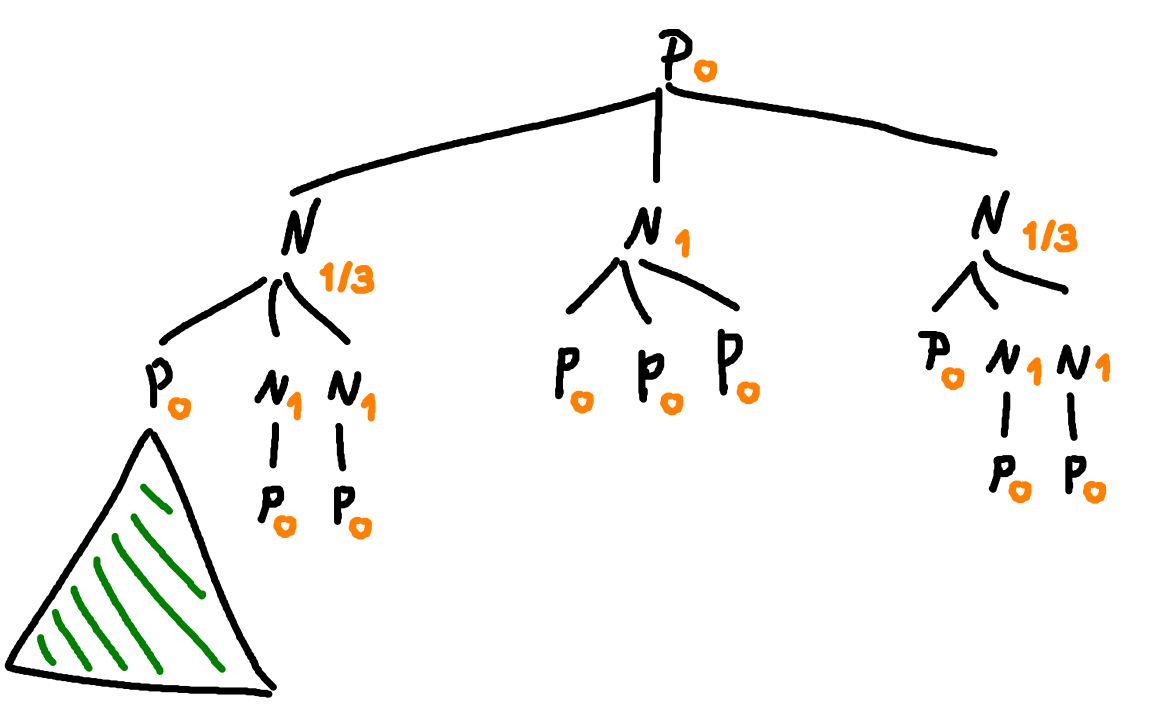
\includegraphics[scale=0.25]{img/ejemplo.png}
    \caption{Ejemplo de dos \nPositions{} con el mismo valor pero distintos sub-árboles}
\end{figure}

Se podría extender el método para que contemple de alguna forma la profundidad del subárbol. 

\section*{Conclusiones y trabajo futuro}

Fue un trabajo práctico muy interesante de implementar. Sobre todo, fue curioso como definiciones tan sencillas llevaron a un juego con un análisis tan complejo.

Como hablamos anteriormente, algo que nos quedó pendiente fue elaborar otro tipo de estrategias para dificultar la elección del otro jugador.

De la mano con esto, nos hubiese gustado elaborar alguna metodología con la cual comparar distintas estrategias. Una idea interesante podría ser armar una especie de torneo entre las distintas estrategias, y ver como se desenvuelven en distintas instancias del juego. Se podrían incluir heurísticas y estrategias de control contra las cuales puedan jugar. Por ejemplo, una que haga movimientos legales aleatorios. Luego, podríamos medir qué tan buenas son comparando el porcentaje de victorias contra cada una (comenzando desde una posición perdedora, para que las óptimas tengan posibilidad de perder).

Por último, queda como trabajo futuro desarrollar un algoritmo que calcule las \calN{} y \calP{} posiciones haciendo uso de los resultados y teoremas del álgebra de juegos definido en clase, en la que se contemplaba la partición de un juego por separado y se analizaba su suma. Aquí probablemente se podría haber utilizado para analizar cada \textit{heap} por separado.

\end{document}